%!TeX root=../sensetop.tex
\chapter[Chapter \thechapter]{}
\lettrine[lines=4,lraise=0.3]{E}{linor} now found the difference between the expectation of an unpleasant event, however certain the mind may be told to consider it, and certainty itself. She now found, that in spite of herself, she had always admitted a hope, while Edward remained single, that something would occur to prevent his marrying Lucy; that some resolution of his own, some mediation of friends, or some more eligible opportunity of establishment for the lady, would arise to assist the happiness of all. But he was now married; and she condemned her heart for the lurking flattery, which so much heightened the pain of the intelligence.

That he should be married soon, before (as she imagined) he could be in orders, and consequently before he could be in possession of the living, surprised her a little at first. But she soon saw how likely it was that Lucy, in her self-provident care, in her haste to secure him, should overlook every thing but the risk of delay. They were married, married in town, and now hastening down to her uncle’s. What had Edward felt on being within four miles from Barton, on seeing her mother’s servant, on hearing Lucy’s message!

They would soon, she supposed, be settled at Delaford.—Delaford,—that place in which so much conspired to give her an interest; which she wished to be acquainted with, and yet desired to avoid. She saw them in an instant in their parsonage-house; saw in Lucy, the active, contriving manager, uniting at once a desire of smart appearance with the utmost frugality, and ashamed to be suspected of half her economical practices;—pursuing her own interest in every thought, courting the favour of Colonel Brandon, of Mrs Jennings, and of every wealthy friend. In Edward—she knew not what she saw, nor what she wished to see;—happy or unhappy,—nothing pleased her; she turned away her head from every sketch of him.

Elinor flattered herself that some one of their connections in London would write to them to announce the event, and give farther particulars,—but day after day passed off, and brought no letter, no tidings. Though uncertain that any one were to blame, she found fault with every absent friend. They were all thoughtless or indolent.

»When do you write to Colonel Brandon, ma’am?« was an inquiry which sprung from the impatience of her mind to have something going on.

»I wrote to him, my love, last week, and rather expect to see, than to hear from him again. I earnestly pressed his coming to us, and should not be surprised to see him walk in today or tomorrow, or any day.«

This was gaining something, something to look forward to. Colonel Brandon \textit{must} have some information to give.

Scarcely had she so determined it, when the figure of a man on horseback drew her eyes to the window. He stopt at their gate. It was a gentleman, it was Colonel Brandon himself. Now she could hear more; and she trembled in expectation of it. But it was \textit{not} Colonel Brandon; neither his air, nor his height. Were it possible, she must say it must be Edward. She looked again. He had just dismounted: she could not be mistaken,—it \textit{was} Edward. She moved away and sat down. »He comes from Mr Pratt’s purposely to see us. I \textit{will} be calm; I \textit{will} be mistress of myself.«

\begin{figure}[tbph]
\centering
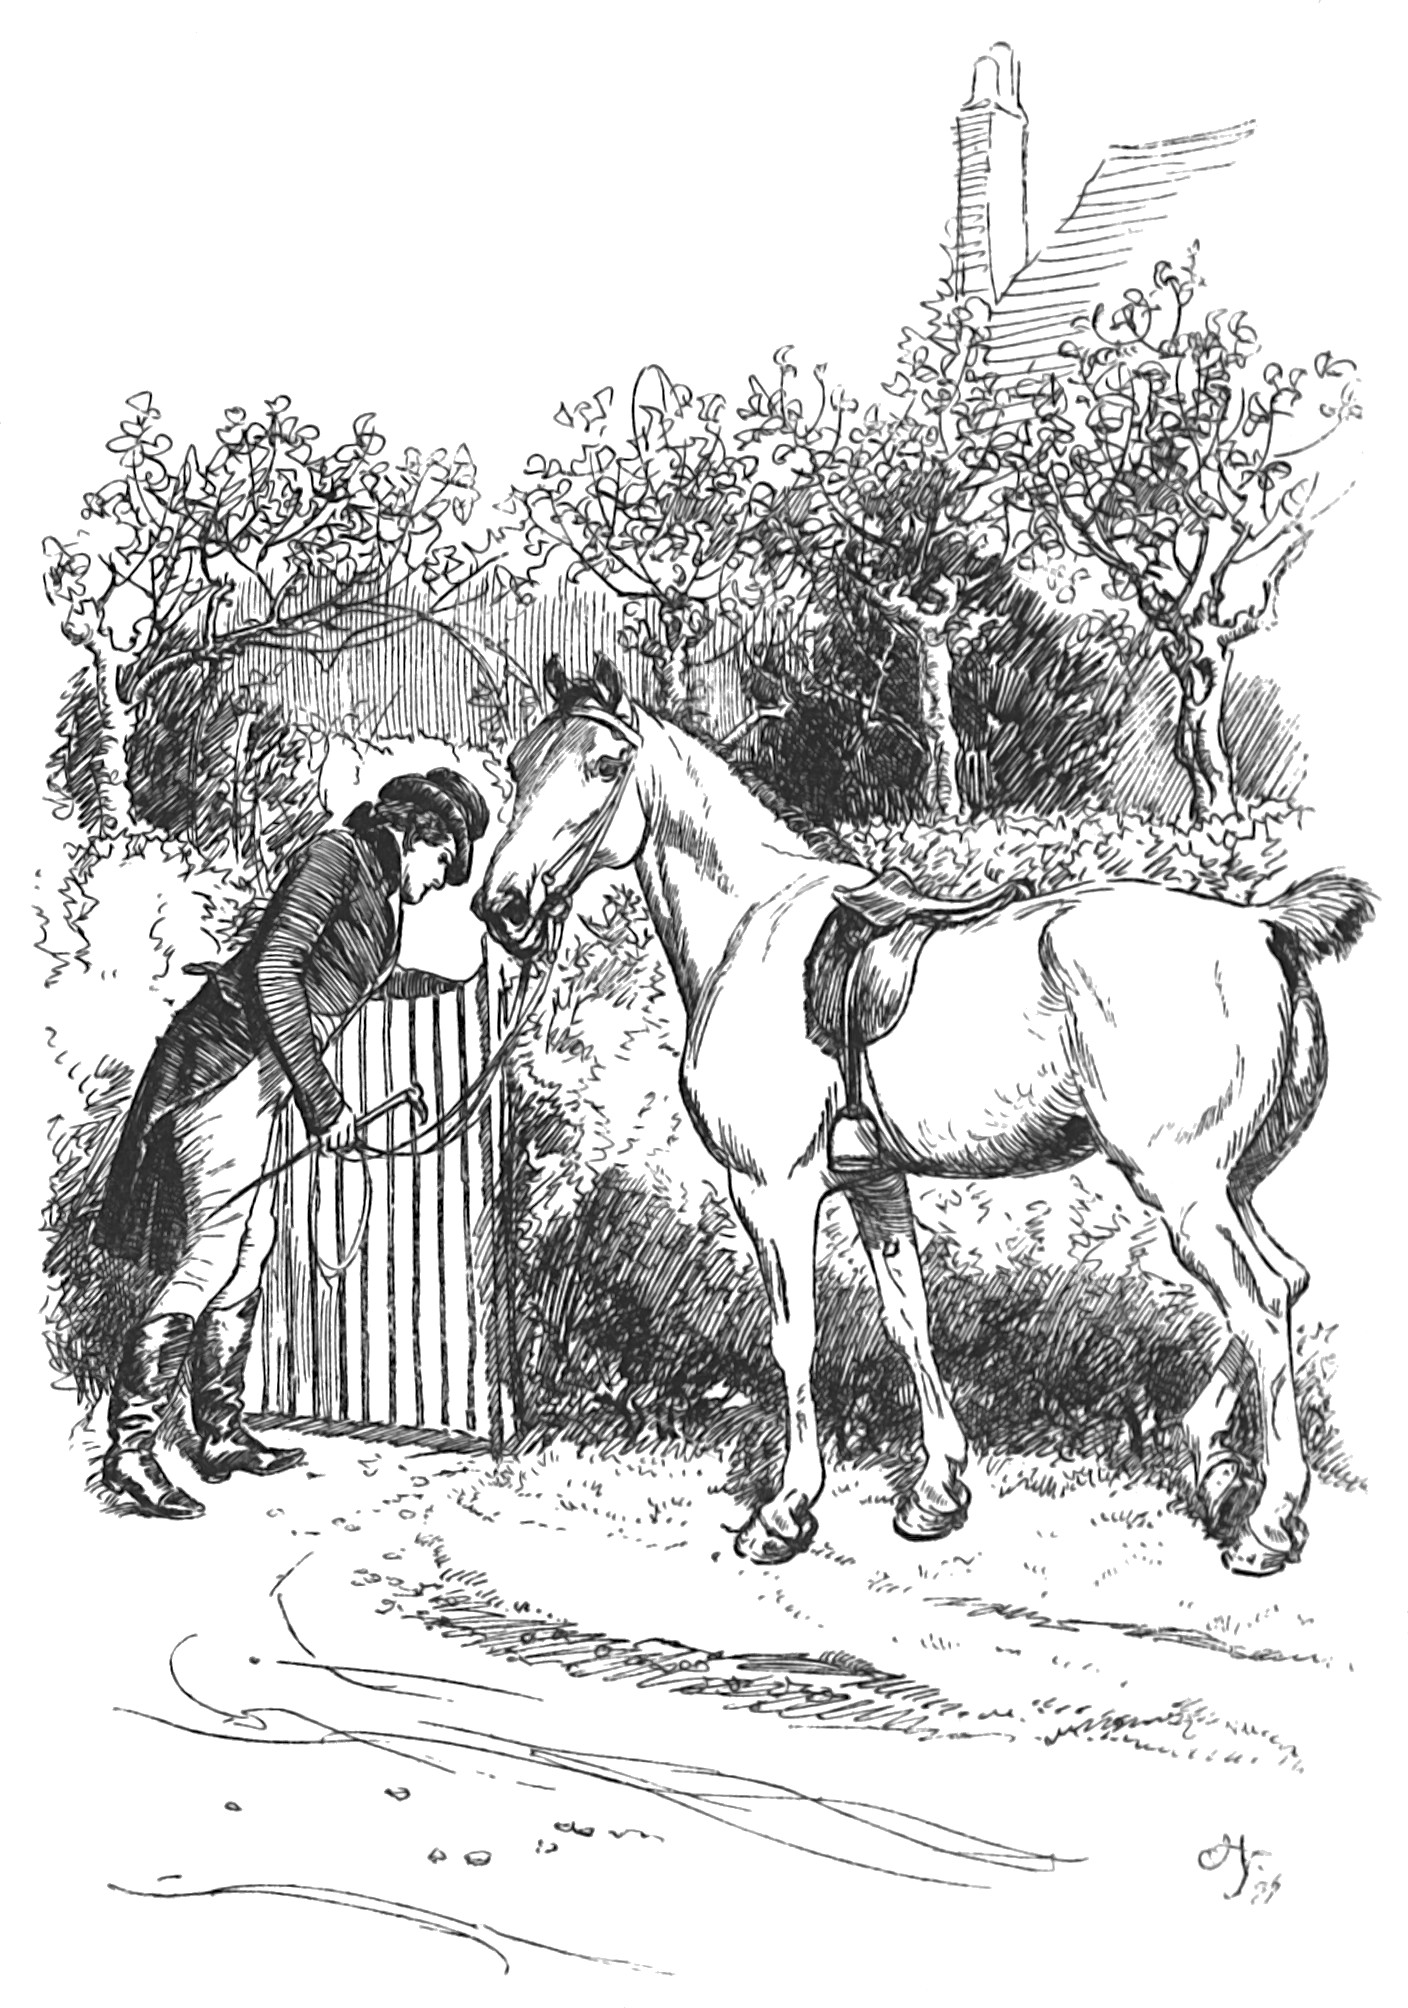
\includegraphics[width=\linewidth]{48edward}
\caption{It \textit{was} Edward}
\end{figure}

In a moment she perceived that the others were likewise aware of the mistake. She saw her mother and Marianne change colour; saw them look at herself, and whisper a few sentences to each other. She would have given the world to be able to speak—and to make them understand that she hoped no coolness, no slight, would appear in their behaviour to him;—but she had no utterance, and was obliged to leave all to their own discretion.

Not a syllable passed aloud. They all waited in silence for the appearance of their visitor. His footsteps were heard along the gravel path; in a moment he was in the passage, and in another he was before them.

His countenance, as he entered the room, was not too happy, even for Elinor. His complexion was white with agitation, and he looked as if fearful of his reception, and conscious that he merited no kind one. Mrs Dashwood, however, conforming, as she trusted, to the wishes of that daughter, by whom she then meant in the warmth of her heart to be guided in every thing, met him with a look of forced complacency, gave him her hand, and wished him joy.

He coloured, and stammered out an unintelligible reply. Elinor’s lips had moved with her mother’s, and, when the moment of action was over, she wished that she had shaken hands with him too. But it was then too late, and with a countenance meaning to be open, she sat down again and talked of the weather.

Marianne had retreated as much as possible out of sight, to conceal her distress; and Margaret, understanding some part, but not the whole of the case, thought it incumbent on her to be dignified, and therefore took a seat as far from him as she could, and maintained a strict silence.

When Elinor had ceased to rejoice in the dryness of the season, a very awful pause took place. It was put an end to by Mrs Dashwood, who felt obliged to hope that he had left Mrs Ferrars very well. In a hurried manner, he replied in the affirmative.

Another pause.

Elinor resolving to exert herself, though fearing the sound of her own voice, now said,

»Is Mrs Ferrars at Longstaple?«

»At Longstaple!« he replied, with an air of surprise. »No, my mother is in town.«

»I meant,« said Elinor, taking up some work from the table, »to enquire for Mrs \textit{Edward} Ferrars.«

She dared not look up;—but her mother and Marianne both turned their eyes on him. He coloured, seemed perplexed, looked doubtingly, and, after some hesitation, said,—

»Perhaps you mean—my brother—you mean Mrs—Mrs \textit{Robert} Ferrars.«

»Mrs Robert Ferrars!« was repeated by Marianne and her mother in an accent of the utmost amazement; and though Elinor could not speak, even \textit{her} eyes were fixed on him with the same impatient wonder. He rose from his seat, and walked to the window, apparently from not knowing what to do; took up a pair of scissors that lay there, and while spoiling both them and their sheath by cutting the latter to pieces as he spoke, said, in a hurried voice,—

»Perhaps you do not know: you may not have heard that my brother is lately married to—to the youngest—to Miss Lucy Steele.«

His words were echoed with unspeakable astonishment by all but Elinor, who sat with her head leaning over her work, in a state of such agitation as made her hardly know where she was.

»Yes,« said he, »they were married last week, and are now at Dawlish.«

Elinor could sit it no longer. She almost ran out of the room, and as soon as the door was closed, burst into tears of joy, which at first she thought would never cease. Edward, who had till then looked any where, rather than at her, saw her hurry away, and perhaps saw—or even heard, her emotion; for immediately afterwards he fell into a reverie, which no remarks, no inquiries, no affectionate address of Mrs Dashwood could penetrate, and at last, without saying a word, quitted the room, and walked out towards the village—leaving the others in the greatest astonishment and perplexity on a change in his situation, so wonderful and so sudden;—a perplexity which they had no means of lessening but by their own conjectures.